\documentclass{article}
\usepackage[utf8]{inputenc}
\usepackage{amssymb}
\usepackage{amsfonts}
\usepackage{amsmath}
\usepackage[utf8]{inputenc}
\usepackage[english]{babel}
\usepackage{lmodern}
\usepackage{float}
\usepackage{graphicx}
\DeclareGraphicsExtensions{.eps,.pdf,.png,.jpg}
\usepackage{latexsym}
\usepackage{hyperref}
\usepackage[euler]{textgreek}
\usepackage{stackengine}
\usepackage{listings}
\usepackage[version-1-compatibility]{siunitx}
\usepackage[usenames,dvipsnames]{xcolor}
\usepackage{pdfpages}
\hypersetup{pdfborder={0 0 0}}
\usepackage{pgfplots}
\pgfplotsset{compat=newest}
\pgfplotsset{plot coordinates/math parser=false}
\newlength\figureheight
\newlength\figurewidth
\usepackage[section]{placeins}%Sørger for at plots og andre floats holder seg til sin section.

\definecolor{dkgreen}{rgb}{0,0.6,0}
\definecolor{gray}{rgb}{0.5,0.5,0.5}
\definecolor{pink}{rgb}{0.63, 0.13, 0.94}
\lstset{language=Matlab, 
    keywords={break, case, catch, continue,else,elseif,end,for,function,
        global,if,otherwise,persistent,return,switch,try,while},
    basicstyle=\ttfamily,
    keywordstyle=\color{blue},
    commentstyle=\color{dkgreen},
    stringstyle=\color{pink},
    numbers=left,
    numberstyle=\tiny\color{gray},
    stepnumber=1,
    numbersep=10pt,
    backgroundcolor=\color{white},
    tabsize=4,
    showspaces=false,
    showstringspaces=false}


\title{Exercise 9 - TTK4130 Modeling and Simulation}
\author{Camilla Sterud}
\date{}

\begin{document}

\maketitle

\newpage

Why on earth does this exercise even exist? What is this supposed to teach anyone except for an absolute bloody hatred for algebra?

\section{Problem 1}

\begin{align*}
    \mathbf{R}_b^a &= 
    \begin{bmatrix}
        \frac{1}{2} \sqrt{3} & -\frac{1}{2} & 0 \\
        \frac{1}{2} & \frac{1}{2} \sqrt{3} & 0 \\
        0 & 0 & 1
    \end{bmatrix}\\
    \mathbf{u}^b &= 
    \begin{bmatrix}
    1\\
    2 \\
    3
    \end{bmatrix},
    \quad 
    \mathbf{w}^a = 
    \begin{bmatrix}
    1\\
    -1 \\
    2
    \end{bmatrix}
\end{align*}



\subsection{a}

We want to show that $\mathbf{R}_b^a$ s a rotational matrix by showing that it is a part of SO3. To show this it is enough to see that 

\begin{align*}
     \mathbf{R}_b^a(\mathbf{R}_b^a)^T &= I =  (\mathbf{R}_b^a)^T\mathbf{R}_b^a\\
     \text{and that}\\
     |\mathbf{R}_b^a| &= 1. 
\end{align*}

\subsection{b}

$\mathbf{R}_b^a$ represents a rotation about the z-axis by $\psi=\arccos{\frac{\sqrt{3}}{2}} = \frac{\pi}{6}$.

\subsection{c}

\begin{equation*}
    \mathbf{R}_a^b = (\mathbf{R}_b^a)^{-1} = (\mathbf{R}_b^a)^T
\end{equation*}

\begin{equation*}
    \underline{\underline{\mathbf{R}_a^b = 
    \begin{bmatrix}
    \frac{1}{2} \sqrt{3} & \frac{1}{2} & 0 \\
    -\frac{1}{2} & \frac{1}{2} \sqrt{3} & 0 \\
    0 & 0 & 1
    \end{bmatrix}}}
\end{equation*}

\subsection{d}

\begin{equation*}
    \underline{\underline{\mathbf{u}^a = \mathbf{R}_b^a\mathbf{u}^b =
    \begin{bmatrix}
    \frac{\sqrt{3}}{2} - 1\\
    \frac{1}{2}+\sqrt{3} \\
    3
    \end{bmatrix}}}
\end{equation*}


\begin{equation*}
    \underline{\underline{\mathbf{w}^b = \mathbf{R}_a^b\mathbf{w}^a =
    \begin{bmatrix}
    \frac{\sqrt{3}}{2} - \frac{1}{2}\\
    \frac{1}{2}-\frac{\sqrt{3}}{2}\\
    2
    \end{bmatrix}}}
\end{equation*}


\subsection{e}

\subsubsection*{i)}

\begin{align*}
    (\mathbf{u}^b)^T\mathbf{w}^b &= (\mathbf{R}_a^b\mathbf{u}^a)^T\mathbf{R}_a^b\mathbf{w}^a\\
                                 &= (\mathbf{u}^a)^T (\mathbf{R}_a^b)^T\mathbf{R}_a^b\mathbf{w}^a\\
                                 &= \underline{\underline{(\mathbf{u}^a)^T\mathbf{w}^a}}
\end{align*}

\subsubsection*{ii)}

\begin{align*}
    (\mathbf{u}^a)^\times\mathbf{w}^a &= \mathbf{u}^a\times\mathbf{w}^a\\
                                      &= (\mathbf{R}_a^b\mathbf{u}^b)\times(\mathbf{R}_a^b\mathbf{w}^b)\\
                                      &= \mathbf{R}_a^b(\mathbf{u}^b\times\mathbf{w}^b)\\
                                      &= \underline{\underline{\mathbf{R}_a^b(\mathbf{u}^b)^\times\mathbf{w}^b}}
\end{align*}

\subsection{f}

Want to calculate $\mathbf{R}_b^a = \mathbf{R}_{z,\psi} \mathbf{R}_{y,\theta} \mathbf{R}_{x,\phi}$.

\begin{align*}
    \mathbf{R}_{z,\psi} &= \begin{bmatrix}
    c\psi & -s\psi & 0 \\
    s\psi & c\psi & 0 \\
    0 & 0 & 1 \\
    \end{bmatrix}\\
    \mathbf{R}_{y,\theta} &= \begin{bmatrix}
    c\theta & 0 & s\theta \\
    0 & 1 & 0 \\
    -s\theta & 0 & c\theta
    \end{bmatrix}\\
    \mathbf{R}_{x,\phi} &= \begin{bmatrix}
    1 & 0 & 0 \\
    0 & c\phi & -s\phi \\
    0 & s\phi & c\phi
    \end{bmatrix} \\
\end{align*}

\begin{equation*}
    \underline{\underline{\mathbf{R}_b^a = 
    \begin{bmatrix}
    c\psi c\theta  & c\psi s\theta s\phi - s\psi c\phi & c\psi s\theta c\phi + s\psi s\phi \\
    s\psi c\theta & s\psi s\theta s\phi + c\psi c\phi &   s\psi s\theta c\phi - c\psi s\theta \\
    - s\theta & c\theta s\phi & c\theta c\phi
    \end{bmatrix}}}
\end{equation*}

\subsection{g}

For $\mathbf{R}_i$ to be in SO(3), they all must have determinant  equal to $1$. All the rows and columns must be unit vectors and must be orthogonal to each other. 
For $\mathbf{R}_1$, this means that 

\begin{align*}
\mathbf{R}_1 &= 
    \begin{bmatrix}
    r_{11} & r_{12} & r_{12} \\
    r_{21} & -1 & r_{23} \\
    r_{31} & r_{32} & 1
    \end{bmatrix}\\
            &= 
    \begin{bmatrix}
    r_{11} & 0 & 0 \\
    0 & -1 & 0 \\
    0 & 0 & 1
    \end{bmatrix}\\
|\mathbf{R}_1| &= r_{11}(-1)\\
\end{align*}

\begin{equation*}
    \underline{\underline{\mathbf{R}_1 = \begin{bmatrix}
    -1 & 0 & 0 \\
    0 & -1 & 0 \\
    0 & 0 & 1
    \end{bmatrix}\\}}.
\end{equation*}

For $\mathbf{R}_2$, this means that 


\begin{align*}
\mathbf{R}_2 &= 
    \begin{bmatrix}
    r_{11} & 1 & r_{13} \\
    r_{21} & r_{22} & r_{23} \\
    r_{31} & r_{31} & 1
    \end{bmatrix}\\
            &= 
    \begin{bmatrix}
    r_{11} & 1 & 0 \\
    r_{21} & 0 & 0 \\
    r_{31} & 0 & 1
    \end{bmatrix}\\
|\mathbf{R}_2| &= -r_{21}\\
\end{align*}

\begin{equation*}
    \underline{\underline{\mathbf{R}_2 = \begin{bmatrix}
    0 & 1 & 0 \\
    -1 & 0 & 0 \\
    0 & 0 & 1
    \end{bmatrix}\\}}.
\end{equation*}

Knowing that 
\begin{equation*}
\mathbf{R}_3 = 
    \begin{bmatrix}
    r_{11} & \frac{1}{\sqrt{3}} & r_{13} \\
    r_{21} & r_{22} & -\frac{1}{2} \\
    \frac{1}{\sqrt{2}} & r_{32} & r_{33}
    \end{bmatrix}
\end{equation*}

leaves us with 

\begin{align*}
    \sqrt{r_{11}^2 + \frac{1}{3} + r_{13}^2} = 1\\
    \sqrt{r_{21}^2 + r_{22}^2 + \frac{1}{4}} = 1\\
    \sqrt{\frac{1}{2} + r_{32}^2 + r_{33}^2} = 1\\
    \frac{1}{\sqrt{3}}r_{11} + r_{21}r_{22} + \frac{1}{\sqrt{2}}r_{32} = 0\\
    \frac{1}{\sqrt{3}}r_{13} -\frac{1}{2}r_{22} + r_{32}r_{33} = 0\\
    r_{11}r_{13} -\frac{1}{2}r_{21} + \frac{1}{\sqrt{2}}r_{33} = 0
\end{align*}

which I am in no way going to solve.


\section{Problem 2}

\subsection{a}

\begin{align*}
    \mathbf{A}_i &= Rot_{z,\theta_i} Trans_{x,d_i} Trans_{x,a_i} Rot_{x,\alpha_i}\\
                 &=\begin{bmatrix} 
                    \mathbf{R}_z(\theta_i) & \mathbf{0} \\
                    \mathbf{0}^T & 1
                    \end{bmatrix}
                    \begin{bmatrix}
                    \mathbf{I} & a_i\mathbf{i}_x\\
                    \mathbf{0} & 1
                    \end{bmatrix}
                    \begin{bmatrix}
                    \mathbf{I} & d_i\mathbf{i}_z \\
                    \mathbf{0} & 1
                    \end{bmatrix}
                    \begin{bmatrix} 
                    \mathbf{R}_z(\theta_i) & \mathbf{0} \\
                    \mathbf{0}^T & 1
                    \end{bmatrix} \\
                 &=\underline{\underline{
                 \begin{bmatrix}
                    c\theta_i  & -s\theta_ic\alpha_i & s\theta_is\alpha_i & a_ic\theta_i \\
                    s\theta_i  & c\theta_ic\alpha_i & -c\theta_is\alpha_i & a_is\theta_i \\
                    0  & s\alpha_i & c\alpha_i & d_i \\
                    0  & 0 & 0 & 1
                 \end{bmatrix}}}
\end{align*}



\subsection{b}

\subsubsection*{Manipilator A}

\begin{equation*}
\underline{\underline{A_1 = 
\begin{bmatrix}
c q_1 & - s q_1 & 0 & l_1 c q_1 \\
s q_1 & c q_1 & 0 & l_1 s q_1 \\
0 & 0 & 1 & 0 \\
0 & 0 & 0 & 1
\end{bmatrix}}}
\end{equation*}


\begin{equation*}
\underline{\underline{A_2 =
\begin{bmatrix}
1 & 0 & 0 & q_2 \\
0 & 1 & 0 & 0 \\
0 & 0 & 1 & 0 \\
0 & 0 & 0 & 1
\end{bmatrix}}}
\end{equation*}

\subsubsection*{Manipulator B}
\begin{equation*}
\underline{\underline{A_1 = 
\begin{bmatrix}
c q_1 & - s q_1 & 0 & l_1 c q_1 \\
s q_1 & c q_1 & 0 & l_1 s q_1 \\
0 & 0 & 1 & 0 \\
0 & 0 & 0 & 1
\end{bmatrix}}}
\end{equation*}

\begin{equation*}
\underline{\underline{A_2 = 
\begin{bmatrix}
c q_2 & - s q_2 & 0 & l_2 c q_2 \\
s q_2 & c q_2 & 0 & l_2 s q_2 \\
0 & 0 & 1 & 0 \\
0 & 0 & 0 & 1
\end{bmatrix}}}
\end{equation*}

\subsection{c}


\subsubsection*{Manipilator A}
\begin{equation*}
\underline{\underline{T^0_2 = A_1 A_2 =
        \begin{bmatrix}
        c q_1 & - s q_1 & 0  & (q_2 + l_1) c q_1 \\
        s q_1 & c q_1   & 0  & (q_2 + l_1) s q_1 \\
        0     & 0       & 1  & 0        \\
        0     & 0       & 0  & 1
        \end{bmatrix}}}
\end{equation*}

\subsubsection*{Manipilator B}

\begin{equation*}
\underline{\underline{T^0_2 = A_1 A_2 =
        \begin{bmatrix}
        c (q_1 + q_2) & - s (q_1 + q_2) & 0  & l_2 c (q_1 + q_2) + l_1 c q_1 \\
        s (q_1 + q_2) & c (q_1 + q_2)   & 0  & l_2 s (q_1 + q_2) + l_1 s q_1 \\
        0     & 0       & 1  & 0        \\
        0     & 0       & 0  & 1
        \end{bmatrix}}}
\end{equation*}

\subsection{d}

Why? Just how is this going to teach anyone anything other than hatred of algebra?
\subsubsection*{Manipilator A}
\begin{equation*}
\underline{\underline{T^0_2 = A_1 A_2 =
        \begin{bmatrix}
        c q_1 - s q_1 + (q_2 + l_1) c q_1 \\
        s q_1 + c q_1   + (q_2 + l_1) s q_1 \\
        1      \\
        1
        \end{bmatrix}}}
\end{equation*}

\subsubsection*{Manipilator B}
\begin{equation*}
    \underline{\underline{g^0 = T^0_2g^2 =
        \begin{bmatrix}
        c (q_1 + q_2) - s (q_1 + q_2) + l_2 c (q_1 + q_2) + l_1 c q_1 \\
        s (q_1 + q_2) + c (q_1 + q_2)   + l_2 s (q_1 + q_2) + l_1 s q_1 \\
        1        \\
        1
        \end{bmatrix}}}
\end{equation*}

\section{Problem 3}

$\mathbf{R} = \mathbf{R_{\mathbf{k},\theta}} = \mathbf{e}^\times + \cos\theta\mathbf{I} + \mathbf{kk}^T(1-\cos\theta)$

\begin{equation*}
    \mathbf{R} = 
    \begin{bmatrix}
    r_{11} & r_{12} & r_{13} \\
    r_{21} & r_{22} & r_{23} \\
    r_{31} & r_{32} & r_{33}
    \end{bmatrix}
\end{equation*}


\subsection{a}

Mikkel was not able to solve this, nor explain why the result was right. If even he can't explain me why the solution is as it is, there is no point in me typing the solution in here just to pretend I understood any of it.

\subsection{b}

Since $\mathbf{R_{\mathbf{k},-\theta}} = -\mathbf{e}^\times + \cos\theta\mathbf{I} + \mathbf{kk}^T(1-\cos\theta)$, $\mathbf{R_{\mathbf{k},\theta}} - \mathbf{R_{\mathbf{k},-\theta}} = 2\mathbf{e}^\times$, and 

\begin{equation*}
    \mathbf{R_{\mathbf{k},\theta}} - \mathbf{R_{\mathbf{k},-\theta}} = 
    \begin{bmatrix}
        0 & -2e_z & 2e_y\\
        2e_z & 0 & -2e_x\\
        -2e_y & 2e_x & 0
    \end{bmatrix}
    = \begin{bmatrix}
        0 & r_{12}-r_{21} & r_{13} - r_{31}\\
        r_{21} - r_{12} & 0 & r_{23} - r_{32}\\
        r_{31} - r_{13} & r_{32} - r_{23} & 0
    \end{bmatrix}
\end{equation*}

we know that 

\begin{equation*}
    \mathbf{e} = \frac{1}{2}\begin{bmatrix}
        r_{32} - r_{23}\\
        r_{13} - r_{31}\\
        r_{21} - r_{12}
    \end{bmatrix}.
\end{equation*}

\subsection{c}

Since $\mathbf{k}$ depends on $sin\theta$, and $\sin\theta$ is $2\pi$ periodic, the rotation will switch both rotational direction and the direction of the axis abiut which it is rotating. This will result in the exact same rotation. 

\subsection{d}

\begin{figure}[H]
    \centering
    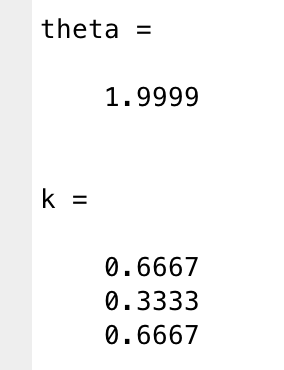
\includegraphics[width = 0.8\textwidth]{ktheta}
    \caption{The output from running the code in Listing \ref{lst:3d}}
\end{figure}

\lstinputlisting[label=lst:3d,caption=Code for finding $\theta$ and $\mathbf{k}$ from a matrix $\mathbf{R}$ in MATLAB., frame = single]{ex9_3d.m}




\end{document}